\chapter{Geometry of smooth and discret curves}
\section{Introduction}

\subsection{Goals and contributions}
Dans ce chapitre, après un bref rappel sur le cadre mathématique d'étude des courbes paramétrique de l'espace, on présente les notions de courbures et de torsion géométrique associées au repère de Frenet. On montre ensuite le cas plus général d'un repère mobile quelconque attaché à une courbe gamma. On définit enfin la particularité d'un repère mobile adapté à un courbe, et on présente, en sus du repère de Frenet, une approche différente pour accrocher des repères le long d'une courbe (Bishop / RMF / Zéro-twisting frame)

\subsection{Related work}
%
%\cite{Bishop1975}
%\cite{Bergou2008}
%\cite{Hoffmann2008}

\subsection{Overview}

% --------------------------------------------------------------------------------------------------------------------------------------------
% SMOOTH SPACE CURVE
% --------------------------------------------------------------------------------------------------------------------------------------------


\section{Paramectric Curves}

% parametric curve
\subsection{Definition}
Let $I$ be an interval of $\mathbb{R}$ and $F\colon t \mapsto F(t)$ be a map of ${\mathcal{C}}^{}(I,{\mathbb{R}}^3)$. Then $\gamma=(I,F)$ is called a \emph{parametric curve} and :
\begin{itemize}
\item The 2-uplet $(I,F)$ is called a \emph{parametrization} of $\gamma$
\item $\gamma = F(I) = \{F(t), t \in I\}$ is called the \emph{graph} or \emph{trace} of $\gamma$
\item $\gamma$ is said to be ${\mathcal{C}}^{k}$ if $F \in {\mathcal{C}^{k}}^{}(I,{\mathbb{R}}^3)$
\end{itemize}

\begin{myrk}
Note that for a given graph in ${\mathbb{R}}^3$ they may be different possible parameterizations. From now, $\gamma$ will simply refer to $F(I)$, its graph.
\end{myrk}

% regularity
\subsection{Regularity}
Let $\gamma=(I,F)$ be a parametric \cite{Bloomenthal} curve, and $t_0 \in I$ a parameter.
\begin{itemize}
\item A point of parameter $t_0$ is called \emph{regular} if $F'(t_0) \neq 0$.
\\The curve $\gamma$ is called \emph{regular} if $\gamma$ is $\mathcal{C}^{1}$ and $F'(t) \neq 0, \forall t \in I$
\item A point of parameter $t_0$ is called \emph{biregular} if $F'(t_0)$ and $F''(t_0)$ are not collinear
\\The curve $\gamma$ is called \emph{biregular} if $\gamma$ is $\mathcal{C}^{2}$ and  $F'(t)\cdot    F''(t) \neq 0, \forall t \in I$
\end{itemize}

% reparametrization
\subsection{Reparametrization}
Let $\gamma=(I,F)$ be a parametric curve of class ${\mathcal{C}}^{k}$, $J \in {\mathbb{R}}^{3}$ an interval, and $\varphi\colon I\mapsto J$ a ${\mathcal{C}}^{k}$ diffeomorphisme. Lets define $G=F\circ\varphi$. Then :
\begin{itemize}
\item $G\in{\mathcal{C}}^{k}(J,{\mathbb{R}}^3)$
\item $G(J)=F(I)$
\item $\varphi$ is said to be an admissible \emph{change of parameter} for $\gamma$
\item  $(J,G)$ is said to be another \emph{admissible parametrization} for $\gamma$
\end{itemize}

% natural parametrization
\subsection{Natural parametrization}
Let $\gamma$ be a space curve of class ${\mathcal{C}}^{1}$. A parametrization $(I,F)$ of $\gamma$ is called \emph{natural} if $\|F'(t)\| = 1, \forall t \in I$. Thus :
\begin{itemize}
\item The curve is necessarily regular
\item F is strictly monotonic
\end{itemize}

% curve length
\subsection{Curve length}
Let $\gamma=(I,F)$ be a parametric curve of class ${\mathcal{C}}^{1}$. The length of $\gamma$ is define as :
\begin{equation}
L=\int_{I}\|F'(t)\|dt
\end{equation}
Note that the length of $\gamma$ is invariant under reparametrization.

% arc-length
\subsection{Arc-length parametrization}
Let $\gamma=(I,F)$ be a regular parametric curve of class ${\mathcal{C}}^{1}$. Let $t_0 \in I$ be a given parameter. The following map is said to be the \emph{arc-length of origin $t_0$} of $\gamma$ :
\begin{equation}
s \colon t \mapsto \int_{t_{0}}^{t}\|F'(u)\|du
\quad,\quad
s \in I \times \mathbb{R}
\end{equation}

The arc-length $s \colon I\mapsto s(I)$ is an admissible change of parameter for $\gamma$. Indeed, $s$ is a ${\mathcal{C}}^{1}$ diffeomorphisme because it is bijective ($s'>0$).

Lets define $G=F\circ s^{-1}$ and $J=s(I)$. Thus $(J,G)$ is a natural reparametrization of $\gamma$ and  $\|G'(s)\| = 1, \forall s \in J$.

This parametrization is preferred because the natural parameter s traverses the image of $\gamma$ at unit speed ($\|G'\| = 1$).


% --------------------------------------------------------------------------------------------------------------------------------------------
% FRENET THRIEDRON
% --------------------------------------------------------------------------------------------------------------------------------------------


\section{Frenet's Trihedron}
\label{sec:frenet}
The trihedron of Frenet is a fundamental mathematical tool from the field of differential geometry to study local characterization of planar and non-planar space curves. It is a direct orthonormal basis attached to a point $P$ sliding along a parametric curve ($\gamma$). Introduced by Jean-Frédéric Frenet in his thesis upon \emph{curves of double curvature} in 1847, it brings out intrinsic local properties of space curves : the curvature ($\kappa$) which evaluates the deviance of $\gamma$ from being a straight line, and the torsion ($\tau$), which evaluates the deviance of $\gamma$ from being a plane curve. These quantities are also known as \guil{generalized curvatures}.
The \emph{fundamental theorem of space curves} states that a curve is fully determined by its curvature and torsion up to a solid (or euclidean) movement in space. This assertion is equivalent to the well-known \emph{Serret-Frenet formulas}, which give the first-order linear differential equations system that govern the evolution of Frenet's trihedron along a space curve. For a given curvature and torsion, and a given initial trihedron, the geometry of the space curve can be constructed by integration these differential equations.

In this section we consider $\gamma=(J,G)$ to be a regular ($\|\gamma'\|=1$) parametric curve of class ${\mathcal{C}}^{2}$, parametrized by its arc-length (denoted $s$). For the sake of simplicity we will refer to $G(s)$ as $\gamma(s)$.

% tangent vector
\subsection{Tangent vector}
The first vector of Frenet's trihedron is called the \emph{unit tangent vector} ($\vect{t}$). At any given parameter $s \in J$,  it is defined as :
\begin{equation}
\vect{t}(s) = \frac{\gamma'(s)}{\|\gamma'(s)\|} = \gamma'(s)
\quad,\quad
\|\vect{t}(s)\|=1
\end{equation}

In differential geometry, the tangente to the curve $\gamma$ at point $P_0$ is obtained as the limit of the (normalized) vector $\overrightarrow{P_0 P}$ , as $P$ approches $P_0$ on the path $\gamma$. For a regular curve, the left-sided and right-sided limits coïncide as $P^-$ and $P^+$ approche $P_0$ respectively from the left and the right sides :
\begin{equation}
	\vect{t}(P_0)
	= \lim_{P \to P_0}\frac{\overrightarrow{P_0 P}}{\norm{\overrightarrow{P_0 P}}}
	= \lim_{P^- \to P_0}\frac{\overrightarrow{P_0 P^-}}{\norm{\overrightarrow{P_0 P^-}}}
	= \lim_{P^+ \to P_0}\frac{\overrightarrow{P_0 P^+}}{\|\overrightarrow{P_0 P^+}\|}
\label{eq:3_4}
\end{equation}

%Normal vector
\subsection{Normal vector}
The second vector of Frenet's trihedron is called the \emph{unit normal vector} ($\vect{n}$). It is constructed from $\vect{t'}$ which is orthogonal to $\vect{t}$. Indeed, $\|\vect{t}\|=1 \Rightarrow \vect{t^{'}} \cdot  \vect{t} = 0 \Leftrightarrow  \vect{t^{'}} \perp \vect{t}$. Thus, at any given parameter $s \in J$, it is defined as :
\begin{equation}
\vect{n}(s) = \frac{\vect{t}'(s)}{\|\vect{t}'(s)\|} = \frac{\gamma''(s)}{\|\gamma''(s)\|}
\quad,\quad
\|\vect{n}(s)\|=1
\end{equation}
Remark that the notion of \guil{normal vector} would be ambiguous for non-planar curves as far as there is an infinite number of possible vectors laying in the plane orthogonal to the curve's tangent. In practice, the tangent derivative is a convenient choice as it allows to extend the notion of curvature from planar to non-planar space curves. The tangent unit vector and the normal unit vector $\{\vect{t},\vect{n}\}$ define the so-called \guil{osculating plane}.

Likewise the differential definition of the tangent exposed in \eqref{eq:3_4}, the osculating plane could be seen as the limit of the plane defined by 3 points $P_0$, $P^-$, $P^+$, as $P^-$ and $P^+$ approches $P_0$ respectively from its left and right side.


%Binormal vector and torsion
\subsection{Binormal vector}
The third vector of Frenet's trihedron is called the \emph{unit binormal vector} ($\vect{b}$). It is constructed from $\vect{t}$ and $\vect{n}$ to form an orthonormal direct basis of $\mathbb{R}^{3}$. Thus, at any given parameter $s \in J$, it is defined as :
\begin{equation}
\vect{b}(s) = \vect{t}(s) \times \vect{n}(s)
\quad,\quad
\|\vect{b}(s)\|=1
\end{equation}
The normal unit vector and the binormal unit vector $\{\vect{n},\vect{b}\}$ define the so-called \guil{normal plane}.
The normal tangent vector and the binormal unit vector $\{\vect{t},\vect{b}\}$ define the so-called \guil{rectifying plane}.

% --------------------------------------------------------------------------------------------------------------------------------------------
% CURVATURE
% --------------------------------------------------------------------------------------------------------------------------------------------

\begin{figure}[t]
\begin{center}
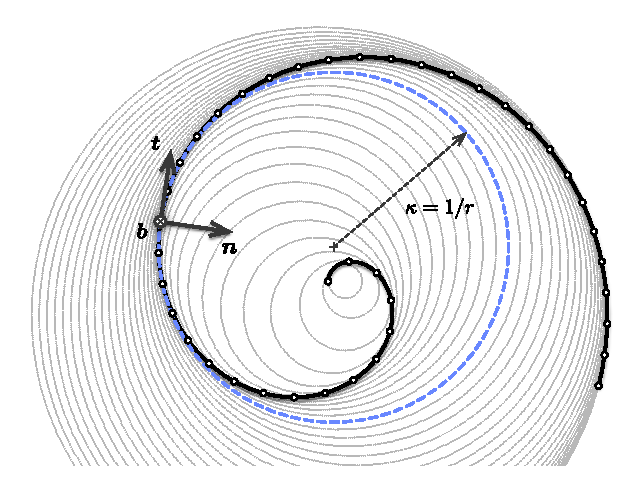
\includegraphics[]{osculating_circle.pdf}
\caption{Different osculating circles for a spiral.}
\label{fig:3_1}
\end{center}
\end{figure}

\begin{figure}[h]
     \centering
     \subfloat[][Tangent.]{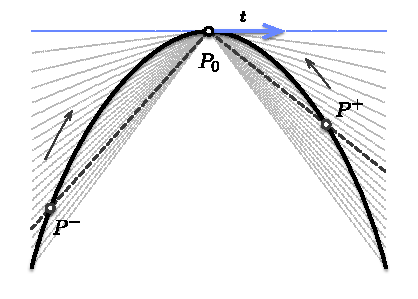
\includegraphics{frenet_tangent.pdf}\label{<figure1>}}
     \subfloat[][Normal and osculating circle]{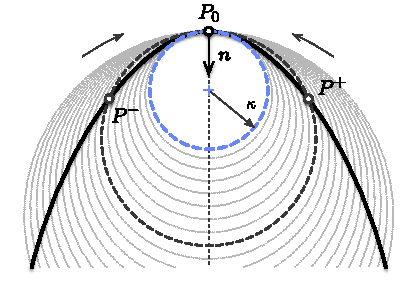
\includegraphics{frenet_normal.pdf}\label{<figure2>}}
     \caption{Differential definition of Frenet's trihedron at given point $P_0$.}
     \label{}
\end{figure}

\section{Curvature}

Note that from a geometric point of view, $\frac{1}{\kappa(s)}$ represents the radius of the osculating circle of $\gamma$ at the point of parameter $s$.

$\kappa(s) = \|\vect{t}'(s)\| = \|\gamma''(s)\|$


How do you know a curve is curving?
And how much?
The answer should depend just on the
shape of the curve, not on the speed at
which it is drawn.
So it connects with
arclength s, not with a time-
parameter t

%Curvature binormal
\subsection{Osculating circle}
Défini de façon directe, le cercle de courbure est le cercle le plus proche de la courbe en P, c'est l'unique cercle osculateur à la courbe en ce point. Ceci signifie qu'il constitue une très bonne approximation de la courbe, meilleure qu'un cercle tangent quelconque. En effet, il donne non seulement une idée de la direction dans laquelle la courbe avance (direction de la tangente), mais aussi de sa tendance à tourner de part ou d'autre de la tangente.

Le centre de courbure est la position limite de l'intersection des deux normales en M(s) et M(s+Ds) et on parle alors de cercle de courbure ou cercle osculateur (du latin osculor, osculatus = caresser).

%Curvature binormal
\subsection{Curvature binormal vector}
Finally, we define the \emph{curvature binormal vector} at any given parameter $s \in J$ as :
\begin{equation}
\vect{\kappa b}(s) = \vect{t}(s) \times \vect{t}'(s) = \kappa(s)\cdot\vect{b}(s)
\quad,\quad
\|\vect{\kappa b}(s)\|= \kappa(s)
\end{equation}

% --------------------------------------------------------------------------------------------------------------------------------------------
% TORSION
% --------------------------------------------------------------------------------------------------------------------------------------------

\begin{figure}[t]
\begin{center}
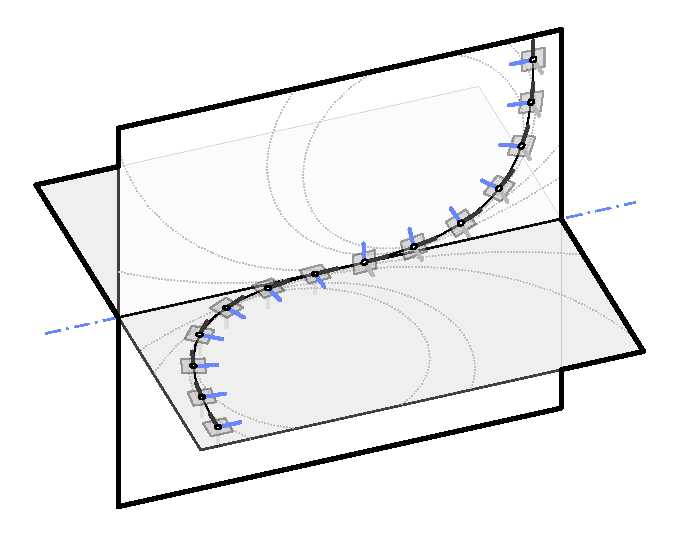
\includegraphics[]{frenet_torsion.pdf}
\caption{Geometric torsion and rotation of the osculating plane}
\label{fig:3_1}
\end{center}
\end{figure}

\section{Torsion}
En géométrie différentielle, la torsion d'une courbe tracée dans l'espace mesure la manière dont la courbe se tord pour sortir de son plan osculateur (plan contenant le cercle osculateur). Ainsi, par exemple, une courbe plane a une torsion nulle et une hélice circulaire est de torsion constante. Prises ensemble, la courbure et la torsion d'une courbe de l'espace en définissent la forme comme le fait la courbure pour une courbe plane. La torsion apparait comme coefficient dans les équations différentielles du repère de Frenet.

The \emph{torsion} measures the deviance of $\gamma$ from being a planar curve and is defined at any given parameter $s \in J$ as :
\begin{equation}
\tau_f(s) = \vect{n}'(s) \cdot \vect{b}(s)
\end{equation}

Cette notion est propre aux courbes gauches et mesure comment la courbe se "tord" en changeant de plan. Dans le trièdre de Frenet, elle correspond à l'angle des plans osculateurs P(s) et P(s + Ds) en deux points infiniment proches M(s) et M(s + Ds), donc à l'angle Dû entre les binormales mesurant comment la courbe se tord en passant de P(s) à P(s + Ds). Ainsi, de façon analogue à la courbure, la torsion T en un point sera, par unité d'arc, la limite lorsque Ds tend vers 0 du rapport Dû/Ds :

%\begin{myprop}
%Si $F$ est ${\mathcal{C}}^{1}$ et régulière alors nécessairement elle est monotone car $F'$ est de signe constant.
%\end{myprop}

%\begin{figure}[t]
%\centering
%\includegraphics[width=\linewidth]{img_ch1_1_frenet.pdf}
%\caption{Repères de Frenet attachés à $\gamma$.}
%\label{fig:1_1}
%\end{figure}


% --------------------------------------------------------------------------------------------------------------------------------------------
% CURVE FRAMING
% --------------------------------------------------------------------------------------------------------------------------------------------


\section{Curve Framing}

% moving frame
\subsection{Moving frame}

Let $\gamma : s \rightarrow \gamma(s)$ be an arc-length parametrized curve. A map $F$ which associates to each point of arc-length $s$ a direct orthonormal trihedron is called a \emph{moving frame} :
\begin{equation}
	\fonctionL{F}{[0,L]}{\mathcal{SO}_{3}(\mathbb{R})}{s}{F(s) = \{\vect{e}_{3}(s),\vect{e}_{1}(s),\vect{e}_{2}(s)\}}
\end{equation}
Thus, inherently, a moving frame $F$ attached to $\gamma$ satisfies for all $s \in [0,L]$ :
\begin{equation}
\begin{cases}
&\| \vect{e}_i(s) \| = 1 \\
&\vect{e}_i(s) \cdot \vect{e}_j(s) = 0\quad , \quad i \neq j
\end{cases}
\end{equation}
The terme \guil{moving frame} will refer indifferently to the map itself ($F$), or to a specific evaluation of the map ($F(s)$).

% governing equations
\subsubsection{Governing equations}
Computing the derivatives of the previous relationships leads to the following differential equations :
\begin{equation}
\begin{cases}
&\vect{e}'_i(s) \cdot \vect{e}_i(s) = 0 \\
&\vect{e}'_{i}(s) \cdot \vect{e}_{j}(s) = -\vect{e}_{i}(s) \cdot \vect{e}'_{j}(s)\quad , \quad i \neq j
\end{cases}
\end{equation}
Thus, there exists 3 scalar functions $\tau(s)$, $k_{1}(s)$, $k_{2}(s)$ such that :
\begin{equation}
\begin{cases}
&\vect{e}'_{3}(s) = k_{2}(s)\vect{e}_{1}(s) - k_{1}(s)\vect{e}_{2}(s) \\
&\vect{e}'_{1}(s) = -k_{2}(s)\vect{e}_{3}(s) + \tau(s)\vect{e}_{2}(s) \\
&\vect{e}'_{2}(s) = k_{1}(s)\vect{e}_{3}(s) - \tau(s)\vect{e}_{1}(s)
\end{cases}
\end{equation}
It is common to rewrite this first-order linear differential equations system as a single matrix equation :
\begin{equation}
	\begin{bmatrix}
		\vect{e}'_{3}(s) \\
		\vect{e}'_{1}(s) \\
		\vect{e}'_{2}(s)
	\end{bmatrix}
	=
	\begin{bmatrix}
		0 & k_{2}(s) & -k_{1}(s) \\
		-k_{2}(s) & 0 & \tau(s) \\
		k_{1}(s) & -\tau(s) & 0
	\end{bmatrix}
	\begin{bmatrix}
		\vect{e}_{3}(s) \\
		\vect{e}_{1}(s) \\
		\vect{e}_{2}(s)
	\end{bmatrix}
\label{eq:3_12}
\end{equation}
Since the progression of any moving frame along $\gamma$ is ruled by a first-order differential equation, a unique triplet $\{\tau, k_{1}, k_{2}\}$ leads to a set of moving frames equal to each other within a constant of integration. Basically, with a given triplet $\{\tau, k_{1}, k_{2}\}$, one would \guil{propagate} a given initial direct orthonormal trihedron (at $s=0$ for instance) through the whole curve by integrating the differential system. In general, a moving frame will be fully determined by $\tau$, $\kappa_{1}$, $\kappa_{2}$ plus $\{\vect{e}_{3}(s=0),\vect{e}_{1}(s=0),\vect{e}_{2}(s=0)\}$.

% vecteur de Darboux
\subsubsection{Darboux vector}
It is relevant to consider the mobile frame's evolution along $\gamma$ introducing the so-called \emph{Darboux vector} ($\vect{\Omega}$), which corresponds to the instantaneous angular velocity of $F$ at each point of arc-length $s$. Thus, the previous differential system governing the evolution of $F(s)$ along $\gamma$ becomes :
\begin{equation}
	\vect{e}'_{i}(s) = \vect{\Omega}(s) \times \vect{e}_{i}(s)
	\quad avec \quad
	\vect{\Omega}(s)
	=
	\begin{bmatrix}
		\tau(s) \\
		k_1(s) \\
		k_2(s)
	\end{bmatrix}
\end{equation}
This result is straightforward deduced from \eqref{eq:3_12}. Note that the cross product \guil{reveals} that the system is skew-symmetric, which could already be seen in \eqref{eq:3_12}.
Geometrically, decomposing the infinitesimal rotation of the moving frame around its directors between arc-length $s$ and $s+ds$ (\autoref{fig:3_2}) shows that the scalar functions $\tau(s)$, $k_{1}(s)$, $k_{2}(s)$ effectively correspond to the angular speed of the frame, respectively around $\vect{e}_{3}(s)$, $\vect{e}_{1}(s)$, $\vect{e}_{2}(s)$ :
\begin{equation}
	\frac{d\theta_3}{dt}(s) = \tau(s)
	\quad,\quad
	\frac{d\theta_1}{dt}(s) = k_{1}(s)
	\quad,\quad
	\frac{d\theta_2}{dt}(s) = k_{2}(s)
\end{equation}

\begin{figure}[t]
\begin{center}
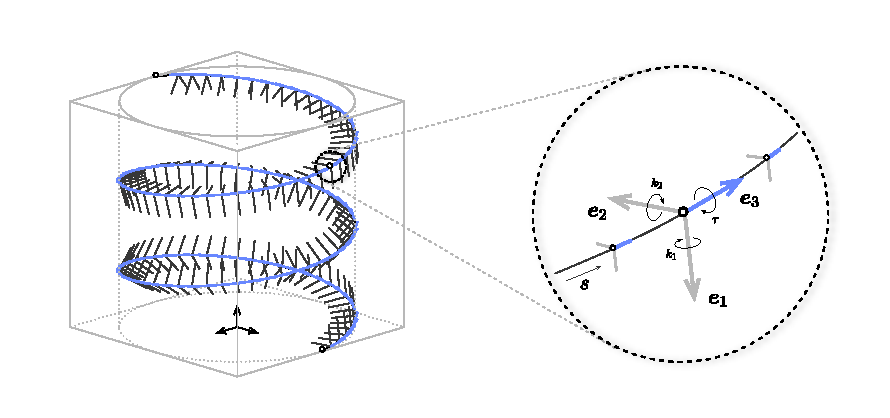
\includegraphics[]{adapted_moving_frame.pdf}
\caption{Adapted moving frame $F(s) =\{\vect{e}_{3}(s),\vect{e}_{1}(s),\vect{e}_{2}(s)\}$ where $\vect{e}_3(s) = \vect{t}(s)$.}
\label{fig:3_1}
\end{center}
\end{figure}

\begin{figure}[t]
\begin{center}
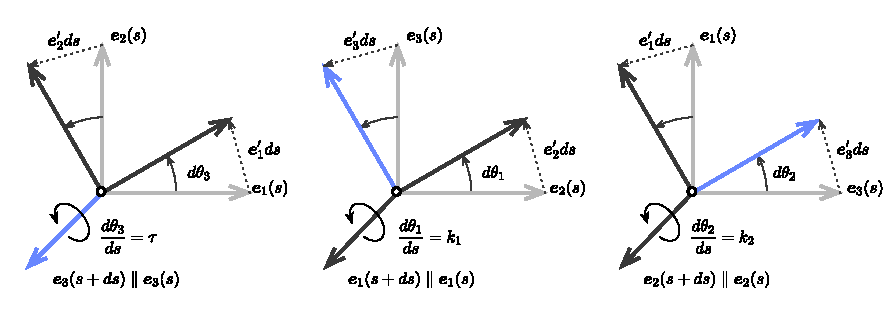
\includegraphics[]{darboux.pdf}
\caption{Geometric interpretation of the Darboux vector of a moving frame.}
\label{fig:3_2}
\end{center}
\end{figure}

% adapted frame
\subsection{Adapted frame}
Let $F$ be a moving frame as defined in the previous section. $F$ is said to be \emph{adapted} to $\gamma$ if at each point $\gamma(s)$, $\vect{e}_{3}(s)$ is tangent to $\gamma$ :
\begin{equation}
	\vect{d_{3}}(s) = \vect{t}(s) = \frac{\gamma^{'}(s)}{\|\gamma(s)\|}, \quad \forall s \in [0,L]
\end{equation}

For an adapted frame, the components $k_1$ and $k_2$ of the Darboux vector are related to the curve's curvature. Indeed, recall from \ref{} that $\kappa \equiv \|\gamma''\| = \|\vect{t}'\|$. Or $\vect{t} = \vect{d}_3$ for an adapted frame. Thus, the following relation holds :
\begin{equation}
	\kappa = \|\vect{d}'_3\| = \sqrt{{k_{1}}^2 + {k_{2}}^2}
\end{equation}
\note{
La courbure est une quantité géométrique intrinsèque, indépendante du choix du repère mobile attaché à la courbe. C'est donc un invariant. Et donc quelque soit le choix du repère mobile adapté $\|\vect{t'}\| = \sqrt{\kappa_1^2 + \kappa_2^2}$ est un invariant (la courbure).

Faire le lien avec l'énergie de flexion, qui ne dépend donc que de la géométrie de la courbe dans le cas d'une isotropic rod $\mathcal{E}_b = EI\kappa^2$.}

% FRENET FRAME
\subsection{Frenet frame}

% definition
\subsubsection{Definition}
The Frenet frame is a well-known particular adapted moving frame (\autoref{sec:frenet}). At any given regular point $\gamma(s)$ it is define as $\{\vect{t}(s),\vect{n}(s),\vect{b}(s)\}$ where :
\begin{gather}
\vect{t}(s) = \frac{\gamma^{'}(s)}{\|\gamma'(s)\|}
\quad,\quad
\vect{n}(s) = \frac{\vect{t'}(s)}{\vect{\kappa}(s)}
\quad,\quad
\vect{b}(s)= \vect{t}(s)\times\vect{n}(s)
\end{gather}

\subsubsection{Governing equations}
The Frenet frame satisfies the \emph{Frenet-Serret} formulas, which govern the evolution of the frame along the curve $\gamma$ :
\begin{gather}
\left[\begin{array}{c}
\vect{t^{'}}(s) \\
\vect{n^{'}}(s) \\
\vect{b^{'}}(s)
\end{array}\right]
=
\left[\begin{array}{ccc}
0 & \kappa_{}(s) & 0 \\
-\kappa_{}(s) & 0 & \tau_f(s) \\
0 & -\tau_f(s) & 0
\end{array}\right]
\left[\begin{array}{c}
\vect{t}(s) \\
\vect{n}(s) \\
\vect{b}(s)
\end{array}\right]
\end{gather}

One can remember the generic differential equations of an adapted moving frame attached to a curve, where :
\begin{gather}
\vect{d_{3}}(s) = \vect{t}(s) = \frac{\gamma^{'}(s)}{\|\gamma(s)\|}
\quad,\quad
\kappa_{1}(s) = 0
\quad,\quad
\kappa_{2}(s) = \kappa(s)
\quad,\quad
\tau(s) = \tau_{f}(s)
\end{gather}



\subsubsection{Darboux vector}
Consequently, the Darboux vector ($\vect{\Omega_{f}}$) of the Frenet frame is given by :
\begin{gather}
\vect{\Omega_f}(s)
=
\left[\begin{array}{c}
\tau_{f}(s) \\
0 \\
\kappa(s)
\end{array}\right]
\end{gather}


\subsubsection{Specific points}

\note{undefined when curvature vanishes : montrer des examples

not related to mechanical torsion

une perturbation de la courbe dans le sens le sens de la courbure engendre une variation de longueur de la courbe proportionnelle à l'inverse de la courbure (au premier ordre) + schéma

une perturbation de la courbe dans le sens de la binormale (en tout point) préserve la longueur de la courbe au 1er ordre : c'est un déplacement qui conserve l'hypothèse d'inextensibilité au premier ordre

Examiner la question de la fermeture sur une boucle fermée. Schéma.
}

% REPERE DE BISHOP
\subsection{Bishop frame}

% definition
\subsubsection{Definition}
Different ways to frame a curve. The usual one is Frenet. But, it could not be as relevant as we want in our field of interest.

The Bishop frame is defined as a a well-known particular adapted moving frame (\autoref{sec:frenet}). At any given regular point $\gamma(s)$ it is define as $\{\vect{t}(s),\vect{n}(s),\vect{b}(s)\}$ where :
\begin{gather}
\vect{t}(s) = \frac{\gamma^{'}(s)}{\|\gamma'(s)\|}
\quad,\quad
\vect{n}(s) = \frac{\vect{t'}(s)}{\vect{\kappa}(s)}
\quad,\quad
\vect{b}(s)= \vect{t}(s)\times\vect{n}(s)
\end{gather}

\subsubsection{Governing equations}
The Bishop frame evolution is governed by the following differential equations :
\begin{gather}
\left[\begin{array}{c}
\vect{t^{'}}(s) \\
\vect{u^{'}}(s) \\
\vect{v^{'}}(s)
\end{array}\right]
=
\left[\begin{array}{ccc}
0 & \kappa_{2}(s) & -\kappa_{1}(s) \\
-\kappa_{2}(s) & 0 & 0 \\
\kappa_{1}(s) & 0 & 0
\end{array}\right]
\left[\begin{array}{c}
\vect{t}(s) \\
\vect{u}(s) \\
\vect{v}(s)
\end{array}\right]
\end{gather}

One can remember the generic differential equations of an adapted moving frame attached to a curve, where :
\begin{gather}
\vect{d_{3}}(s) = \vect{t}(s) = \frac{\gamma^{'}(s)}{\|\gamma(s)\|}
\quad,\quad
\kappa_{1}(s) = 0
\quad,\quad
\kappa_{2}(s) = \kappa(s)
\quad,\quad
\tau(s) = \tau_{f}(s)
\end{gather}

\subsubsection{Darboux vector}
Consequently, the Darboux vector ($\vect{\Omega_{b}}$) of the Bishop frame is given by :
\begin{gather}
\vect{\Omega_b}(s)
=
\left[\begin{array}{c}
0\\
\kappa_1(s)\\
\kappa_2(s)
\end{array}\right]
\end{gather}

\subsubsection{Specific points}
well defined when curvature vanishes

related to mechanical torsion

\note{expliquer la relation entre bishop et frenet : bishop est obtenu par rotation d'un angle $\alpha = \int \tau_f$ par rapport à frenet.

expliquer la notion de parallèle comme l'a formulé Laurent Hauswirth : la projection de $u'$ et $v'$ dans le plan normal à la tangente $t$ est nulle, cad que d'un plan à un autre la projection de $u$ et $v$ est conservée + faire schéma.

Laurent Hauswirth : la complexité d'un problème est en général proportionnelle à la codimension de l'objet étudié et donc, de ce fait les courbes ($codim = 3-1 = 2$) sont des objets plus compliqués que les surfaces ($codim = 3-2=1$) ds $\mathbb{R}^3$.

Expliquer le défaut de fermeture sur une boucle fermée. Calcul du writhe. Quelle différence avec Frenet ?
}

\subsection{Comparison between Frenet and Bishop frames}

\subsubsection{Example A : circular helix}
\begin{equation}
	\left\{
	\begin{array}{c}
		\rho = a\\
		z = b\theta
	\end{array}\right.
\end{equation}

\subsubsection{Example B : conical helix (spiral)}
\begin{equation}
	\left\{
	\begin{array}{c}
		\rho = a e^{k\theta}\\
		z = \rho \cot{\alpha}\\
	\end{array}\right.
\end{equation}


soit pour une spirale dont on connait

\begin{figure}[H]
\centering
\subfloat[][Frenet frame]{%
  \begin{tikzpicture}
\begin{axis}[
	width = 7.5cm,
	xmin=-0.1, xmax= 1.1, restrict x to domain = 0 : 1,
	ymin=-4e-2, ymax= 7e-2, restrict y to domain = -4e-2:6e-2,
	ytick={-3e-2, 0, 3e-2, 6e-2},
	grid=major,
	]

 	\pgfplotstableread{ch3_geometry/plot/frenet_bishop_darboux/frenet.txt}\frenet;
	\addplot [Tblue, smooth, thick]
       	table [x expr=\thisrowno{0}, y expr=\thisrowno{2}] {\frenet};

	\pgfplotstableread{ch3_geometry/plot/frenet_bishop_darboux/frenet.txt}\frenet;
	\addplot [black, smooth, thick, dashed]
       	table [x expr=\thisrowno{0}, y expr=\thisrowno{3}] {\frenet};

	\pgfplotstableread{ch3_geometry/plot/frenet_bishop_darboux/frenet.txt}\frenet;
	\addplot [black, smooth, thick]
       	table [x expr=\thisrowno{0}, y expr=\thisrowno{4}] {\frenet};

\end{axis}
  \end{tikzpicture}}\quad
\subfloat[][Bishop frame]{%
  \begin{tikzpicture}
\begin{axis}[
	width = 7.5cm,
	xmin=-0.1, xmax= 1.1, restrict x to domain = 0 : 1,
	ymin=-4e-2, ymax= 7e-2, restrict y to domain = -4e-2:6e-2,
	ytick={-3e-2, 0, 3e-2, 6e-2},
	grid=major,
	]

       	\pgfplotstableread{ch3_geometry/plot/frenet_bishop_darboux/bishop.txt}\bishop;
	\addplot [Tblue, smooth, thick]
         table [x expr=\thisrowno{0}, y expr=\thisrowno{2}] {\bishop};

         \pgfplotstableread{ch3_geometry/plot/frenet_bishop_darboux/bishop.txt}\bishop;
	\addplot [black, smooth, thick, dashed]
         table [x expr=\thisrowno{0}, y expr=\thisrowno{3}] {\bishop};

         \pgfplotstableread{ch3_geometry/plot/frenet_bishop_darboux/bishop.txt}\bishop;
	\addplot [black, smooth, thick]
         table [x expr=\thisrowno{0}, y expr=\thisrowno{4}] {\bishop};


\end{axis}
  \end{tikzpicture}}
\caption[]{Comparison between Frenet and Bishop frame velocity for a spirale curve.}
\label{g:nognot}
\end{figure}




\section{Discrete Curvature}

\subsection{Definition}

\cite{Hoffmann2008}

The edge osculating circle.
The vertex osculating circle.
La localité est meilleur dans le cas du vertex-based discret osculating circle.
Pour des anlges élevés, le edge-based discret osculating circle est plus pertinent.
La courbure tend vers l'infini quand les 2 edges deviennent colineaires.

La définition du plan osculateur est univoque dans le cas discret : c'est localement le plan défini par 2 edges consécutifs.

Ce n'est pas le cas de la courbure qui perd son côté intrinsèque.

courbure discrete dans le cas général

\subsubsection{Vertex-based osculating circle}

\begin{equation}
	\kappa_1 = \frac{2 \,sin(\varphi_i)}{\|\vect{e}_{i-1} + \vect{e}_{i} \|},
\end{equation}

\begin{figure}[]
\begin{center}
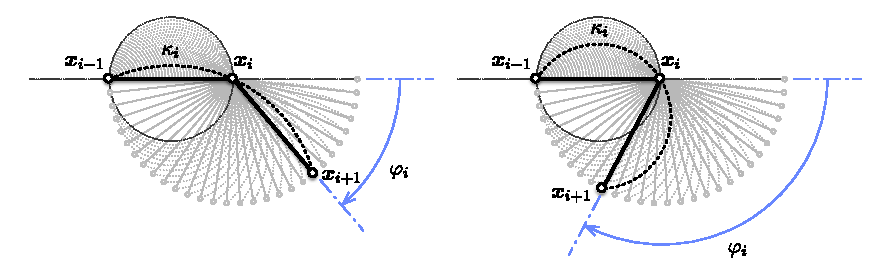
\includegraphics[]{curvature_vertex.pdf}
\caption{Variation of the vertex-based discrete curvature.}
\label{fig:1_1}
\end{center}
\end{figure}

\subsubsection{Edge-based osculating circle}

\begin{equation}
	\kappa_2 = \frac{4 \,tan(\varphi_i/2)}{\|\vect{e}_{i-1}\| + \|\vect{e}_{i} \|}
\end{equation}

\begin{figure}[]
\begin{center}
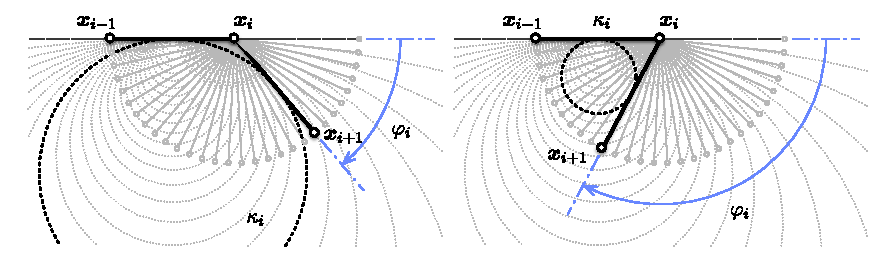
\includegraphics[]{curvature_edge.pdf}
\caption{Variation of the edge-based discrete curvature.}
\label{fig:1_1}
\end{center}
\end{figure}



\begin{figure}[h]
     \centering
     \subfloat[][vertex-based osculating circle]{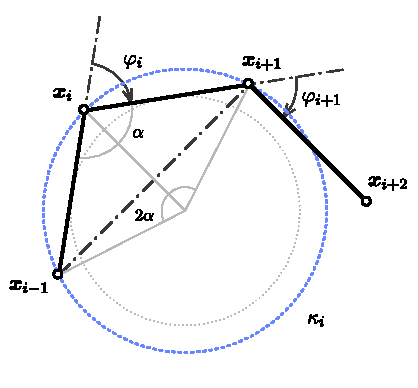
\includegraphics{osculating_circle_vertex.pdf}\label{<figure1>}}
     \subfloat[][edge-based osculating circle]{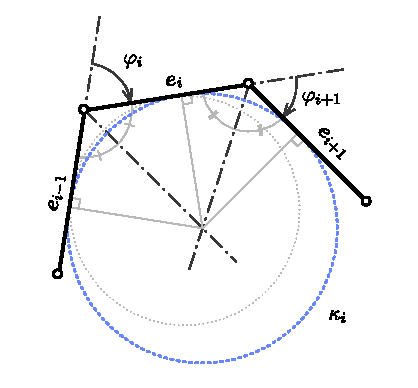
\includegraphics{osculating_circle_edge.pdf}\label{<figure2>}}
     \caption{Definition of the osculating circle for discrete curves.}
     \label{steady_state}
\end{figure}

\begin{figure}[H]
\begin{center}
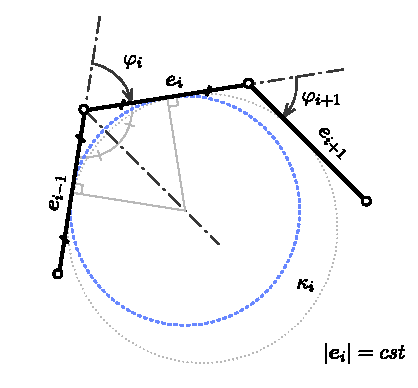
\includegraphics[]{osculating_circle_edge_cst.pdf}
\caption{Another definition of the osculating circle for arc-length parametrized curves.}
\label{fig:1_1}
\end{center}
\end{figure}

\subsection{Variability of discrete curvature regarding $\alpha$}

Qu'on réécrit en posant $\|\vect{e}_{i-1}\| = \alpha \|\vect{e}_{i} \|$, $\alpha \geq 0$ :

\begin{equation}
	\kappa_1 = \frac{2 \,sin(\varphi_i)}{\|\vect{e}_{i}\|(1+ \alpha^2 + 2 \alpha \, cos(\varphi_i))^{1/2}},
	\quad
	\kappa_2 = \frac{4 \,tan(\varphi_i/2)}{\|\vect{e}_{i}\|(1+\alpha)}
\end{equation}

\begin{equation}
	\frac{\kappa_1}{\kappa_2}(\alpha) = \frac{\kappa_1}{\kappa_2}(1/\alpha)= \frac{1+\alpha}{(1+ \alpha^2 + 2 \alpha \, cos(\varphi_i))^{1/2}} \, cos^2(\varphi_i/2)
\end{equation}

\begin{figure}[H]
\begin{center}
\begin{tikzpicture}
\begin{axis}[
	scale only axis,
	legend style={at={(axis cs:0,6)},anchor=north west},
	xmin=-3.1416/4/4, xmax= 3.1416+3.1416/4/4, restrict x to domain = 0 : 3.1416,
	ymin=-2/4, ymax= 10+2/4, restrict y to domain = 0 : 10,
	grid=major,
	axis y line*= left,% the '*' avoids arrow heads
	xlabel={$\varphi$},
	xtick={0, 0.7854, 1.5708, 2.3562, 3.14159},
    	xticklabels={$0$, $\frac{\pi}{4}$,  $\frac{\pi}{2}$,  $\frac{3\pi}{4}$,$\pi$},
	ylabel={$\kappa_1, \kappa_2$},
	ytick={0, 2, 4, 6, 8,10} ]

		% kappa 1
		\addplot[black, samples = 100, domain = 0: 3.1416, solid,  thick]
		{2*sin(deg(x)/2)};
		\node[style={font=\scriptsize}] at (axis cs:3.0,2.4) {$\kappa_1$};
		\addplot[Tgray, samples = 100, domain = 0:3.1416, solid, very thin]					{\curvatureA(deg(x),2)};
		\addplot[color=Tgray, samples = 100, domain = 0:3.1416, solid, very thin]
		{\curvatureA(deg(x),0.5)};

		% kappa 2
		\addplot[black, samples = 400, domain = 0:3.1416, solid,  thick]
		{\curvatureB(deg(x),1)};
		\node[style={font=\scriptsize}] at (axis cs:3.0,9.5) {$\kappa_2$};
		\addplot[color=Tgray, samples = 400, domain = 0:3.1416, solid, very thin]
		{\curvatureB(deg(x),2)};
		\addplot[color=Tgray, samples = 400, domain = 0:3.1416, solid, very thin]
		{\curvatureB(deg(x),0.5)};


	\end{axis}
	\begin{axis}[
	scale only axis,
	xmin=-3.1416/4/4, xmax= 3.1416+3.1416/4/4, restrict x to domain = 0 : 3.1416,
	ymin=-0.2/4, ymax= 1+0.2/4, restrict y to domain = 0 : 1,
	axis y line*=right,
	axis x line=none,
%	ylabel style = {rotate=-90},
	ylabel = {${\kappa_1}/{\kappa_2}$},
	ytick={0, 0.2, 0.4, 0.6, 0.8, 1}
	]
		\addplot[Tblue, samples = 500, domain = 0:3.1416, solid, thick]
		{\curvatureRap(deg(x),1)};
		\node[style={font=\scriptsize}] at (axis cs:1.1,0.95) {$\kappa_1/\kappa_2$};
		\addplot[Tblue, samples = 500, domain = 0:3.1416, solid, very thin]
		{\curvatureRap(deg(x),2)};
	\end{axis}
\end{tikzpicture}

\end{center}
\caption{Discrete curvature comparison for $\alpha \in [0.5,2]$}
\end{figure}

\subsection{Convergence benchmark $\kappa_1$ vs. $\kappa_2$}

\subsubsection{Straight line}

\subsubsection{Circle}

Smooth curve settings:
\begin{equation}
	\mathcal{E} = \int_0^l \kappa^2 ds = \kappa \pi,
	\quad
	l = \pi r,
	\quad
	\kappa = \frac{1}{r}
\end{equation}

Discrete curve :
\begin{equation}
	\varphi_N = \tfrac{\pi}{N},
	\quad
	|\vect{e}| = 2r\sin \tfrac{\varphi}{2},
	\quad
	l_N = N|\vect{e}| =2Nr\sin \tfrac{\varphi}{2} = l \frac{\sin \tfrac{\varphi}{2}}{\tfrac{\varphi}{2}}
\end{equation}

Discrete bending energies :
\begin{equation}
	\mathcal{E}_1 = \mathcal{E} \frac{\sin \tfrac{\varphi}{2}}{\tfrac{\varphi}{2}},
	\quad
	\mathcal{E}_2 = \mathcal{E} \frac{\sin \tfrac{\varphi}{2}}{\tfrac{\varphi}{2} \cos^2 \tfrac{\varphi}{2}},
\end{equation}

Remarque that ratios are independent of scale change (independent of R)

\begin{figure}[H]
\begin{center}
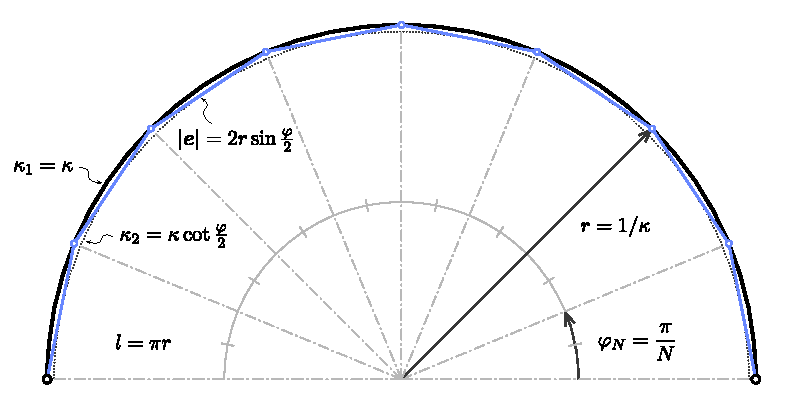
\includegraphics[]{circle.pdf}
\caption{Another definition of the osculating circle for arc-length parametrized curves.}
\label{fig:1_1}
\end{center}
\end{figure}

qsmldkqsmldk s qsd qsd
 sqd
  qs dqs=dlk qs=ldk sq
\newpage
\begin{figure}[]
\begin{center}
\begin{tikzpicture}
	\begin{axis}[
	scale only axis,
	xmin=0, xmax= 21, restrict x to domain = 1 : 20,
	ymin=0.5, ymax= 1.7, restrict y to domain = 0 :1.6,
	grid=major,
	xlabel={$\mathcal{E}_i/\mathcal{E} = f_i(N=l/|e|)$},
	xtick={1,5,10,15,20},
	ylabel={},
	]
		\addplot[black, samples = 1000, domain = 1: 21, solid,  thin]
		{sin(deg(pi/(2*x)))/(pi/(2*x))};
		\node[style={font=\scriptsize}] at (axis cs:3.5,1.565) {$\mathcal{E}_1/\mathcal{E}$};

		\addplot[black, samples = 1000, domain = 1: 21, solid,  thin, dashed]
		{sin(deg(pi/(2*x)))/((pi/(2*x))*cos(deg(pi/(2*x)))^2)};
		\node[style={font=\scriptsize}] at (axis cs:2.5,0.65) {$\mathcal{E}_2/\mathcal{E}$};

		\addplot[Tblue, samples = 1000, domain = 0: 21, solid,  thick]
		{1};
	\end{axis}
\end{tikzpicture}
\end{center}
\caption{Discrete curvature comparison for $\alpha \in [0.5,2]$}
\end{figure}

\subsubsection{Elastica}

\begin{figure}[H]
\begin{center}
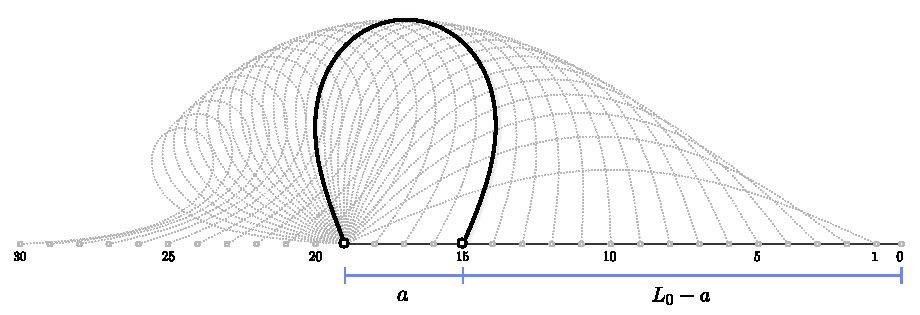
\includegraphics[]{elastica_withnum.pdf}
\caption{Another definition of the osculating circle for arc-length parametrized curves.}
\label{fig:1_1}
\end{center}
\end{figure}

\begin{figure}[H]
\begin{center}
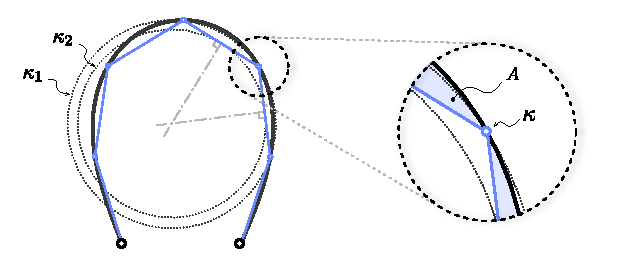
\includegraphics[]{elastica_detail.pdf}
\caption{Another definition of the osculating circle for arc-length parametrized curves.}
\label{fig:1_1}
\end{center}
\end{figure}

\begin{figure}[H]
\centering
\subfloat[][$\mathcal{E}_1/\mathcal{E} = f(N = l/|e|)$]{%
  \begin{tikzpicture}
\begin{axis}[
	width = 7.5cm,
	xmin=8, xmax= 52, restrict x to domain = 10 : 50,
	ymin=0.915, ymax= 1.005, restrict y to domain = 0 :1.6,
	grid=major,
	xtick={0,3,5,10,15,20,25,30,35,40,45,50},
	]

       	\pgfplotstableread{ch3_geometry/plot/discrete_curvature_bench/elastica5.txt}\crvB;
	\addplot [black, smooth, very thin]
       	table [x expr=\thisrowno{0}, y expr=\thisrowno{3}] {\crvB};
%  	\node[Tgray, style={font=\scriptsize}] at (axis cs:9,1) {$5$};

       	\pgfplotstableread{ch3_geometry/plot/discrete_curvature_bench/elastica10.txt}\crvC;
	\addplot [black, smooth, very thin]
        	table [x expr=\thisrowno{0}, y expr=\thisrowno{3}] {\crvC};
    	\node[Tgray, style={font=\scriptsize}] at (axis cs:10,0.985) {$10$};

        \pgfplotstableread{ch3_geometry/plot/discrete_curvature_bench/elastica15.txt}\crvD;
	\addplot [black, smooth, very thin]
         table [x expr=\thisrowno{0}, y expr=\thisrowno{3}] {\crvD};
         \node[Tgray, style={font=\scriptsize}] at (axis cs:10,0.978) {$15$};

     	\pgfplotstableread{ch3_geometry/plot/discrete_curvature_bench/elastica20.txt}	\crvE;
	\addplot [black, smooth, very thin]
       	table [x expr=\thisrowno{0}, y expr=\thisrowno{3}] {\crvE};
       	\node[Tgray, style={font=\scriptsize}] at (axis cs:10,0.965) {$20$};

     	\pgfplotstableread{ch3_geometry/plot/discrete_curvature_bench/elastica25.txt}	\crvF;
	\addplot [black, smooth, very thin]
       	table [x expr=\thisrowno{0}, y expr=\thisrowno{3}] {\crvF};
       	\node[Tgray, style={font=\scriptsize}] at (axis cs:10,0.94) {$25$};

     	\pgfplotstableread{ch3_geometry/plot/discrete_curvature_bench/elastica30.txt}	\crvG;
	\addplot [black, smooth, very thin]
        	table [x expr=\thisrowno{0}, y expr=\thisrowno{3}] {\crvG};
       	\node[Tgray, style={font=\scriptsize}] at (axis cs:15,0.92) {$30$};

         \addplot[Tblue, samples = 100, domain = 0: 50, solid,  thick]
	{1};
\end{axis}
  \end{tikzpicture}}\quad
\subfloat[][$\mathcal{E}_2/\mathcal{E} = f(N = l/|e|)$]{%
  \begin{tikzpicture}
\begin{axis}[
	width = 7.5cm,
	xmin=8, xmax= 52, restrict x to domain = 10 : 50,
	ymin=0.995, ymax= 1.085, restrict y to domain = 1 :1.6,
	grid=major,
	xtick={0,3,5,10,15,20,25,30,35,40,45,50},
	]

         \pgfplotstableread{ch3_geometry/plot/discrete_curvature_bench/elastica5.txt}\crvB;
	\addplot [black, smooth, very thin]
         table [x expr=\thisrowno{0}, y expr=\thisrowno{4}] {\crvB};
         \node[Tgray, style={font=\scriptsize}] at (axis cs:10,1.024) {$5$};

        \pgfplotstableread{ch3_geometry/plot/discrete_curvature_bench/elastica10.txt}\crvC;
	\addplot [black, smooth, very thin]
         table [x expr=\thisrowno{0}, y expr=\thisrowno{4}] {\crvC};
         \node[Tgray, style={font=\scriptsize}] at (axis cs:10,1.044) {$10$};

         \pgfplotstableread{ch3_geometry/plot/discrete_curvature_bench/elastica15.txt}\crvD;
	\addplot [black, smooth, very thin]
         table [x expr=\thisrowno{0}, y expr=\thisrowno{4}] {\crvD};
         \node[Tgray, style={font=\scriptsize}] at (axis cs:10,1.07) {$15$};

     	\pgfplotstableread{ch3_geometry/plot/discrete_curvature_bench/elastica20.txt}	\crvE;
	\addplot [black, smooth, very thin]
         table [x expr=\thisrowno{0}, y expr=\thisrowno{4}] {\crvE};
         \node[Tgray, style={font=\scriptsize}] at (axis cs:13.5,1.08) {$20$};

     	\pgfplotstableread{ch3_geometry/plot/discrete_curvature_bench/elastica25.txt}	\crvF;
	\addplot [black, smooth, very thin]
         table [x expr=\thisrowno{0}, y expr=\thisrowno{4}] {\crvF};
         \node[Tgray, style={font=\scriptsize}] at (axis cs:18,1.08) {$25$};

     	\pgfplotstableread{ch3_geometry/plot/discrete_curvature_bench/elastica30.txt}	\crvG;
	\addplot [black, smooth, very thin]
         table [x expr=\thisrowno{0}, y expr=\thisrowno{4}] {\crvG};
         \node[Tgray, style={font=\scriptsize}] at (axis cs:27,1.08) {$30$};

         \addplot[Tblue, samples = 100, domain = 0: 50, solid,  thick]
	{1};
\end{axis}
  \end{tikzpicture}}
\caption[]{Bending energy representativity}
\label{g:nognot}
\end{figure}

%
%
%\bibliographystyle{alpha}
%\bibliography{../bibliography}
